\section{A detailed explanation of the attributes of the data}

\subsection*{Describe if the attributes are discrete/continous, Nominal/Ordinal/Interval/Ratio.}
	\begin{enumerate}
	\item X - Discrete, Nominal
	\item Y - Discrete, Nominal
	\item month - Discrete, Ordinal
	\item day - Discrete, Ordinal
	\item FFMC - Continous, Interval
	\item DMC - Continous, Interval
	\item DC - Continous, Interval
	\item ISI - Continous, Interval
	\item temp - Continous, Interval
	\item RH - Continous, Ratio
	\item wind - Continous, Ratio
	\item rain - Continous, Ratio
	\item area - Continous, Ratio
	\end{enumerate}
\subsection*{Give an account of whether there are data issues (i.e. missing values or corrupted data) and describe them if so.}
There is no missing values or corrupted data.
\subsection*{Describe the basic summary statistics of the attributes.}
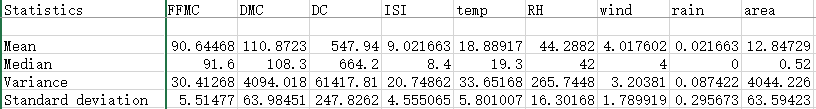
\includegraphics[width=\textwidth]{summary_statistics.png}